\documentclass{article}
\usepackage{amsmath}
\usepackage{setspace}

\usepackage{graphicx}
\graphicspath{{images/}}
\usepackage{wrapfig}
\usepackage{comment}
\usepackage{listings}
\usepackage{xcolor}
\usepackage{float}
%\usepackage[style=numeric]{biblatex}
%\addbibresource{fish.bib}
\usepackage{comment}

\definecolor{codegreen}{rgb}{0,0.6,0}
\definecolor{codegray}{rgb}{0.5,0.5,0.5}
\definecolor{codepurple}{rgb}{0.58,0,0.82}
\definecolor{backcolour}{rgb}{0.95,0.95,0.92}
 
\lstdefinestyle{mystyle}{
    backgroundcolor=\color{backcolour},
    commentstyle=\color{codegreen},
    keywordstyle=\color{magenta},
    numberstyle=\tiny\color{codegray},
    stringstyle=\color{codepurple},
    basicstyle=\fontsize{10}{12}\ttfamily,
    breakatwhitespace=false,
    breaklines=true,
    %breaklines=false,
    captionpos=b,
    keepspaces=true,
    numbers=left,
    numbersep=5pt,
    showspaces=false,
    showstringspaces=false,
    showtabs=false,
    tabsize=2
}
 
\lstset{style=mystyle}

\makeatletter
\renewcommand\section{\clearpage\newpage\@startsection {section}{1}{\z@}%
	{-3.5ex \@plus -1ex \@minus -.2ex}%
	{2.3ex \@plus.2ex}%
	{\normalfont\Large\bfseries}}
\makeatother

\newlength{\mylen}
\definecolor{darkRed}{rgb}{0.6,0,0}
\newcommand{\yf}[1]{{\color{darkRed}{#1}}}

\begin{document}

%==========================================================================
%==========================================================================
% Title pages.

%\begin{comment}
\newcommand{\mytitle}{Automatic Fish Tracking: 
Keeping Track of Who’s Who}
\newcommand{\myauthor}{Ari Spraggins}

\newcommand{\myskip}{\vspace{0.5in}}
\newcommand{\layouttitle}[1]{{\bf\large\MakeUppercase{#1}}}
\setlength{\parindent}{0em}
\doublespace
\pagenumbering{roman}
\thispagestyle{empty}

\begin{center}

	\vspace{4in} 
	\layouttitle{\mytitle} \\ by \\ \myauthor
	
	\vspace{1in}
	A Thesis Submitted to the Faculty of \\
	The Wilkes Honors College \\
	in Partial Fulfillment of the Requirements for the Degree of \\
	Bachelor of Science in Liberal Arts and Sciences \\
	with a Concentration in Physics \\ 
	\vspace{1in} 
	Wilkes Honors College of \\
	Florida Atlantic University \\
	Jupiter, Florida \\
	May \number\year

\end{center}

\newpage

%==========================================================================

\vspace{4in}
\begin{center}
	\layouttitle{\mytitle} \\
	by \\
	\myauthor
\end{center}

\singlespace
\vspace{1in}
This thesis was prepared under the direction of the candidate's thesis advisor, Dr. Yaouen Fily, and has been approved by the members of their supervisory committee. It was submitted to the faculty of the Harriet L. Wilkes Honors College and was accepted in partial fulfillment of the requirements for the degree of Bachelor of Science in Liberal Arts and Sciences.

\vspace{1in}
SUPERVISORY COMMITTEE:

\newcommand{\myrule}{\vspace{0.5in}\rule{4in}{0.5pt} \\}

\myrule
Dr. Yaouen Fily 

\myrule 
Prof. Annina Ruest

\myrule
Dean Justin Perry, Harriet L. Wilkes Honors College 

\myrule
Date

\newpage

%==========================================================================

%\begin{center}
%	\layouttitle{Acknowledgements}
%\end{center}
%\section*{Acknowledgements}
%%\addcontentsline{toc}{section}{Acknowledgements}
%
%\myskip
%Some acknowledgements.
%
%\newpage

%==========================================================================

%\begin{center}
%	\layouttitle{Abstract}
%\end{center}
\section*{Abstract}
\addcontentsline{toc}{section}{Abstract}

\myskip
\renewcommand{\arraystretch}{1.5}
\begin{tabular}{@{}l@{\hspace{3ex}}l}
	Author: & \myauthor \\
	Title: & \mytitle \\
	Institution: & Harriet L. Wilkes Honors College, Florida Atlantic University \\
	Thesis Advisor: & Dr. Yaouen Fily \\
	Degree: & Bachelor of Science in Liberal Arts and Sciences \\
	Concentration: & Physics \\
	Year: & \the\year
\end{tabular}

\myskip
\doublespace
%\end{comment}
Automatic video tracking has had a major impact on animal behavior studies. One of the challenges of this technique is keeping track of the identities of the fish, especially when they swim together and exchange positions. In this project we use the python programming language to address this problem for groups of fish. The video data comes from schooling assays performed at FAU's Cavefish Trilab (Dr. Keene, Dr. Duboue, and Dr. Kowalko). The method is inspired by the idTracker animal tracking software: we track patterns of brightness as a visual identifier of each fish which we then use to detect when the fish swap places.
\newpage

%\begin{comment}
%==========================================================================

\tableofcontents

%\listoftables

\listoffigures

\newpage

%==========================================================================
%\end{comment}

\setlength{\parindent}{1em}
\pagenumbering{arabic}
%\singlespace

%==========================================================================
%==========================================================================
% Thesis proper.


\section{Introduction}

\subsection{Tracking Animal Behaviour}
While visually pleasing, schooling is a rather challenging topic that has long intrigued animal scientists. In order to quantify the animals' behavior, a vast quantity of positional data is needed; more than can be collected by hand. Advances in computer vision technology now make this type of data accessible through computerized video-tracking. Beyond schooling, this allows to quantify a wide variety of behaviors in a very accurate manner.

This thesis focuses on tracking the motion of Mexican Tetra fish (\textit{Astyanax mexicanus}). One of the quirks of the Mexican Tetra species is that some of its populations have been living in underground caves for about a million years. There, they have evolved a number of behavioral differences with the populations living on the surface, including the loss of schooling: whereas surface populations of \emph{A. mexicanus} school, cave-adapted ones do not~\cite{kowalko_utilizing_2020}. 

The data used in this thesis comes from experiments performed on campus in the labs of Dr. Keene, Dr. Dubou\'e, and Dr. Kowalko, collectively known as the Cavefish Trilab. The tracking software that the project aims to improve on was developed by Dr. Fily's group for the Cavefish Trilab~\cite{patch_kinematic_2020, patch_patchmemorycvtracer_2020}. The current version of that software has trouble maintaining the identities of the fish throughout an experiment. The purpose of this work is to fix that issue.

\subsection{Nature of the problem}

Before discussing how to maintain the identity of the fish as we track them, we must first talk a little about how the software locates them. Throughout the thesis {\bf we focus on two-fish experiments}. 
In each frame of the video, the software identifies regions that are darker than their surrounding. After filtering out dark regions whose size of aspect ratio is inconsistent with a fish, each remaining dark spot is interpreted as a fish. This works well for determining the positions of the fish at any given moment, but the identities of the fish can swap (fish 1 becomes fish 2 and vice versa) at any time.

\begin{figure}[H]
	\centering
	\setlength{\mylen}{0.32\linewidth}
	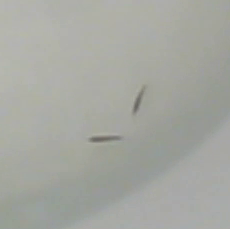
\includegraphics[height=\mylen]{140cropped}%
	\hspace{0.01\linewidth}%
	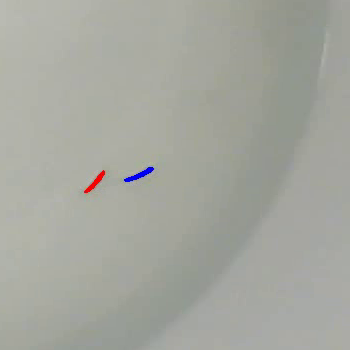
\includegraphics[height=\mylen]{simple-swap1}%
	\hspace{0.01\linewidth}%
	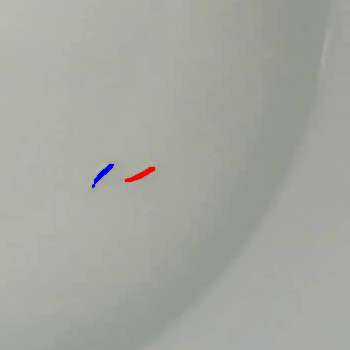
\includegraphics[height=\mylen]{simple-swap2}
	\caption{\emph{Left}: Close-up of two fish in their tank. The tank is made of white plastic. Each fish appears as a dark spot. \emph{Middle and Right}: Two consecutive frames of a two-fish video. Fish 1 is highlighted in blue. Fish 2 is highlighted in red. Basic dark spot detection makes no attempt to maintain the color ID of the fish, i.e., the colors can swap at any time.}
	\label{fig:fish}
\end{figure}

Many of those identity swaps can be fixed by analyzing the distance traveled by each fish. The videos are shot at 30 frames per second, so fish do not move much from one frame to the next. Therefore, the correct ID of a dark spot can often be obtained by matching each dark spot in the frame to the closest dark spot in the previous frame.

%\begin{figure}[H]
%	\centering
%	\setlength{\mylen}{0.32\linewidth}
%	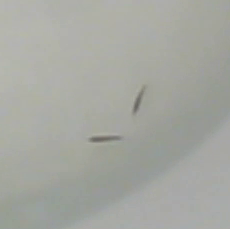
\includegraphics[height=\mylen]{140cropped}%
%	\caption{Left: Close-up of two fish in their tank. The tank is made of white plastic. Each fish appears as a dark spot. Middle and Right: Two consecutive frames of a two-fish video. Fish 1 is highlighted in blue. Fish 2 is highlighted in red. Basic dark spot detection makes no attempt to maintain the color ID of the fish, i.e., the colors can swap at any time.}
%	\label{fig:fish}
%\end{figure}

However, this does not always work. Issues occur in two scenarios: when the fish get close enough that the program thinks there is only one fish (figure~\ref{fig:overlap-event}), and when the fish move fast enough that they are closer to the other's previous position then their previous position. The first of these issues is the easier of the two to check, since it is fairly trivial to check for regions in which only one fish is reported (please see Appendix~\ref{appendix1}). While it is easy enough to check for the first of these issues, the second is a little tougher. To check for errors in these cases, the distance of each fish from its previous position must be compared to the distance from each fish to the other fishes previous position (Appendix~\ref{app:swapStatus}). If the software mistakes the positions of the fish, which we will refer to as a swap, it will look like the fish traveled longer than it should have.



If the fish are near each other and moving fast, then a fish may closer to the previous position of another fish than to its own previous position. In that case, the distance-based method will swap the two fish's identities. 
If the fish are even closer, or if one is over or under another, the algorithm may only detect a single large dark spot. We call this an overlap event. An example is shown in Figure~\ref{fig:overlap-event}. Eventually, the fish separate and the algorithm detects them as distinct dark spots again, but the fish identities are lost in the process and 
\begin{figure}[H]
	\centering
	\setlength{\mylen}{0.32\linewidth}
	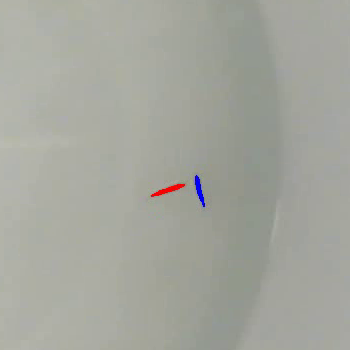
\includegraphics[height=\mylen]{overlap-event1}%
	\hspace{0.01\linewidth}%
	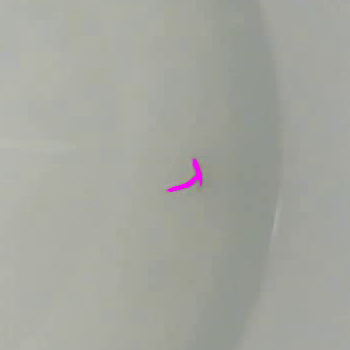
\includegraphics[height=\mylen]{overlap-event2}%
	\hspace{0.01\linewidth}%
	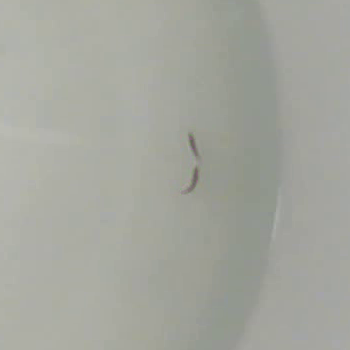
\includegraphics[height=\mylen]{overlap-event3}
	\caption{Overlap event. 
		\emph{Left}: Before the overlap, fish 1 (blue) is on the right and fish 2 (red) is on the left. 
		\emph{Middle}: During the overlap, the dark spot detection algorithm only detects one object (purple). The identities of the fish are meaningless because the algorithm thinks they are at the exact same place. 
		\emph{Right}: After the overlap, the fish identities cannot be recovered by analyzing the distance traveled.}
	\label{fig:overlap-event}
\end{figure}



\subsection{Previous work}

Video-tracking software designed with multi-animal experiments in mind typically handle the first type of identity swap described above -- the ones that are fixable by analyzing the distance traveled between frames. Swaps caused by overlap situations are trickier. Some older video-tracking software offer the possibility to fix the animals' tracks by hand after running the automatic tracking. A popular example is the commercial video-tracking software Ethovision, made by Noldus. The downside of this approach is that it is slower. In some cases, fixing all identity swaps by hand can become the most time-consuming part of the project. 

In recent years, several new software have come out to address this issue using various strategies.

The one this thesis is most heavily inspired from is idTracker~\cite{perez-escudero_idtracker_2014}. The idea is that each fish has a unique pattern of brighter and darker spots on its body, which can be used to recognize the fish even after loosing its track for a while. To quantify those patterns, the program measures spatial brightness correlations over each fish's body and compare them with previous frames to decide whether an identity swap has occurred. A more recent version of this software, known as idTracker.ai, uses machine learning methods to perform this task.

More recently, TRex~\cite{walter_trex_2021} provides a similar workflow but uses deep-learning methods to identify a visual pattern unique to each fish.

DeepLabCut~\cite{mathis_deeplabcut_2018} also uses deep-learning methods, however it solves a more ambitious problem: tracking multiple points of interest on each animal in order to quantify their posture as well as their position. The trade-off here is that the user has to manually identify the points of interest in several frames across the video, which is a bit more labor-intensive.

\subsection{Roadmap}

The goal of this project is to draw from the original idTracker approach to help fix identity swaps in a pre-existing video-tracking code designed for use in Cavefish Trilab: cvtracer~\cite{patch_kinematic_2020, patch_patchmemorycvtracer_2020}. To do this, we will be covering the two processes we use to determine whether or not the fish have been correctly identified depending on how many fish are detected. These two processes are a distance based unswapping method (section~\ref{sec:Distance Based Unswapping}), and a histogram based method (sections~\ref{sec:Histogram Based Unswapping} and~\ref{sec:Histogram Based Unswapping 2}). We will then go over how accurate each of these methods were at giving the fish the correct identity (sections~\ref{sec:Determining Accuracy} and~\ref{sec:Results}).

\section{Methods}

\subsection{Video Collection}
While any actual experimentation on the fish is beyond the scope of this thesis, it is still useful to describe the process of gathering data. The basic setup of the labs we are taking data from is a tank with two fishes in it and a camera trained on them, as seen below. 
This setup produces a video for us to use, of which an example frame is shown below.

\begin{figure}[H]
	\centering
	\setlength{\mylen}{0.35\linewidth}
	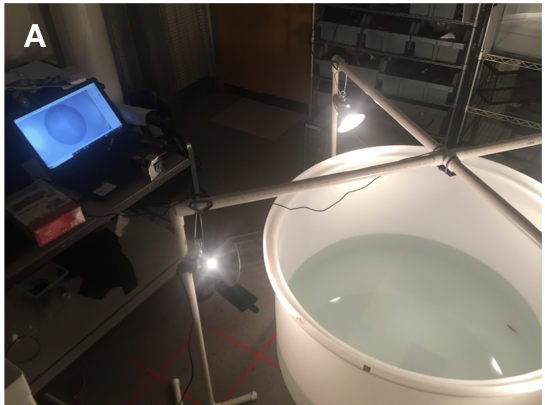
\includegraphics[height=\mylen]{experimental_design}
	\hspace{0.01\linewidth}
	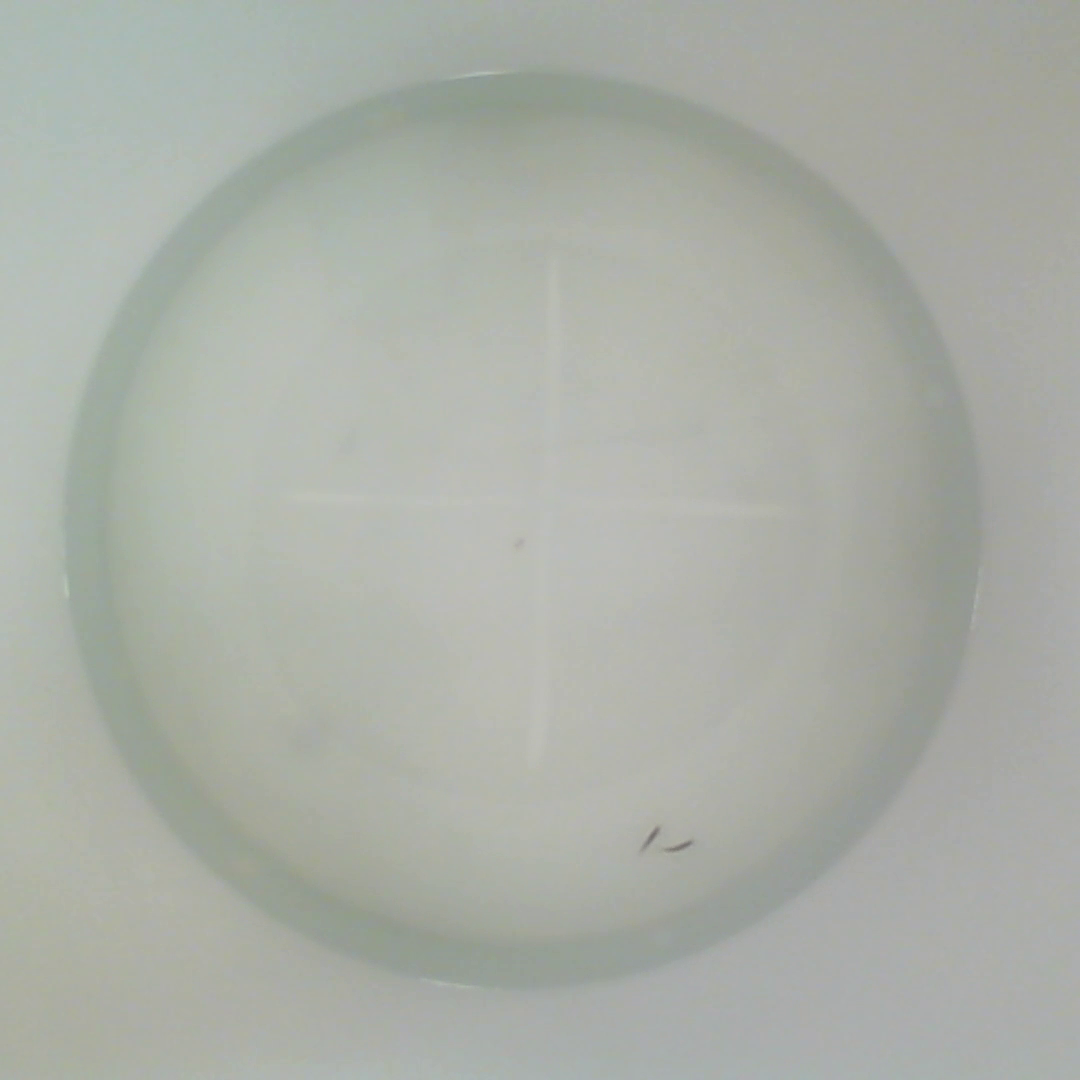
\includegraphics[height=\mylen]{figures.frame5140}
	\caption{\emph{Left}: The tank setup. \emph{Right}: An example frame of the video.}
\end{figure}

\subsection{Current Tracking}

To track the fish, we must first feed the video captured from this setup to an analysis program, in our case cvtracer~\cite{patch_kinematic_2020, patch_patchmemorycvtracer_2020}, which has been especially created for use by the Jupiter Trilab. 
The tracker works taking the tank as a constant background, and noting that the fish are the only dark spots on the tank. It then returns an array for each of the fish containing a list of the fish's pixels and those pixel's colors. Once we have the fish saved in a format that we can analyze, we are ready to start working on the tracking of the fish. Since each the way we store the data gives each fish an identifier, we then can use those identifiers to analyse the fish.

%The next step is to segment the data into regions based on the number of fish it detects. We do this because the distance based unswapping approach doesn't work on regions where there is only one fish detected, so we need to tell the program where it can use that approach.
%
%\begin{figure}[H]
%	\centering
%	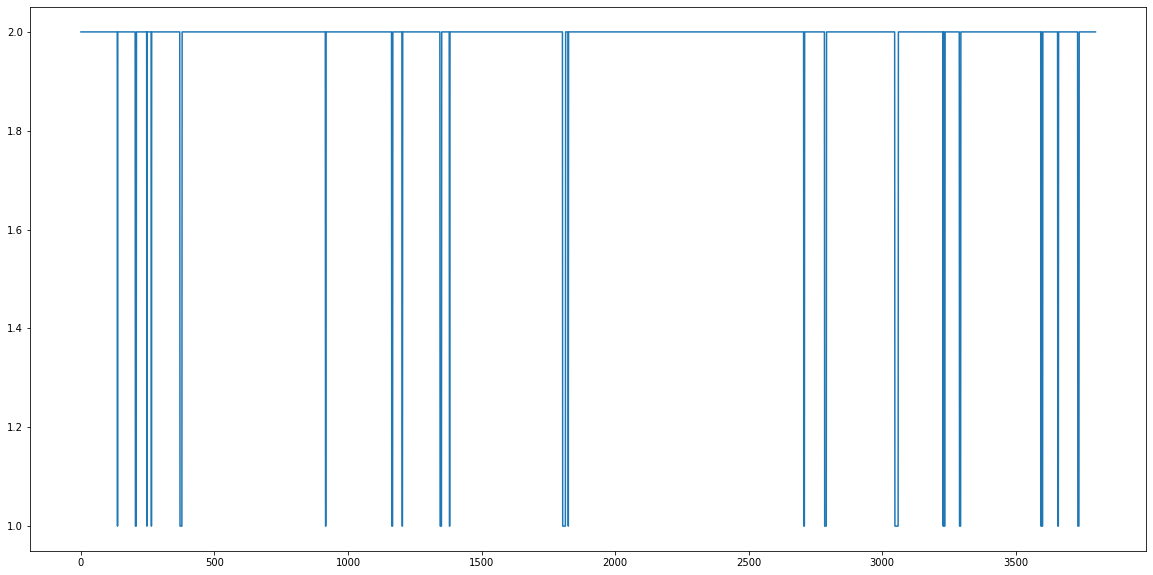
\includegraphics[width=.75\linewidth]{oneFish}
%	\caption{Number of one fish regions}
%\end{figure}


\subsection{Distance Based Unswapping}
\label{sec:Distance Based Unswapping}

The first and simplest round of identity unswapping works by minimizing the total distance traveled by the fish between the previous frame and the current one. Figure~\ref{fig:distance-unswap-principle} illustrates the way the method works for two fish. The semi-transparent fish indicate each fish's position in the previous frame. In the left panel, identities are maintained, and the distances traveled (double arrows) are small. In the right panel, an identity swap has occurred: in the new frame, the red fish has become blue and vice versa. Because of this swap, each fish appears to have traveled much more distance (double arrows) than it actually has.

\begin{figure}[H]
	\centering
	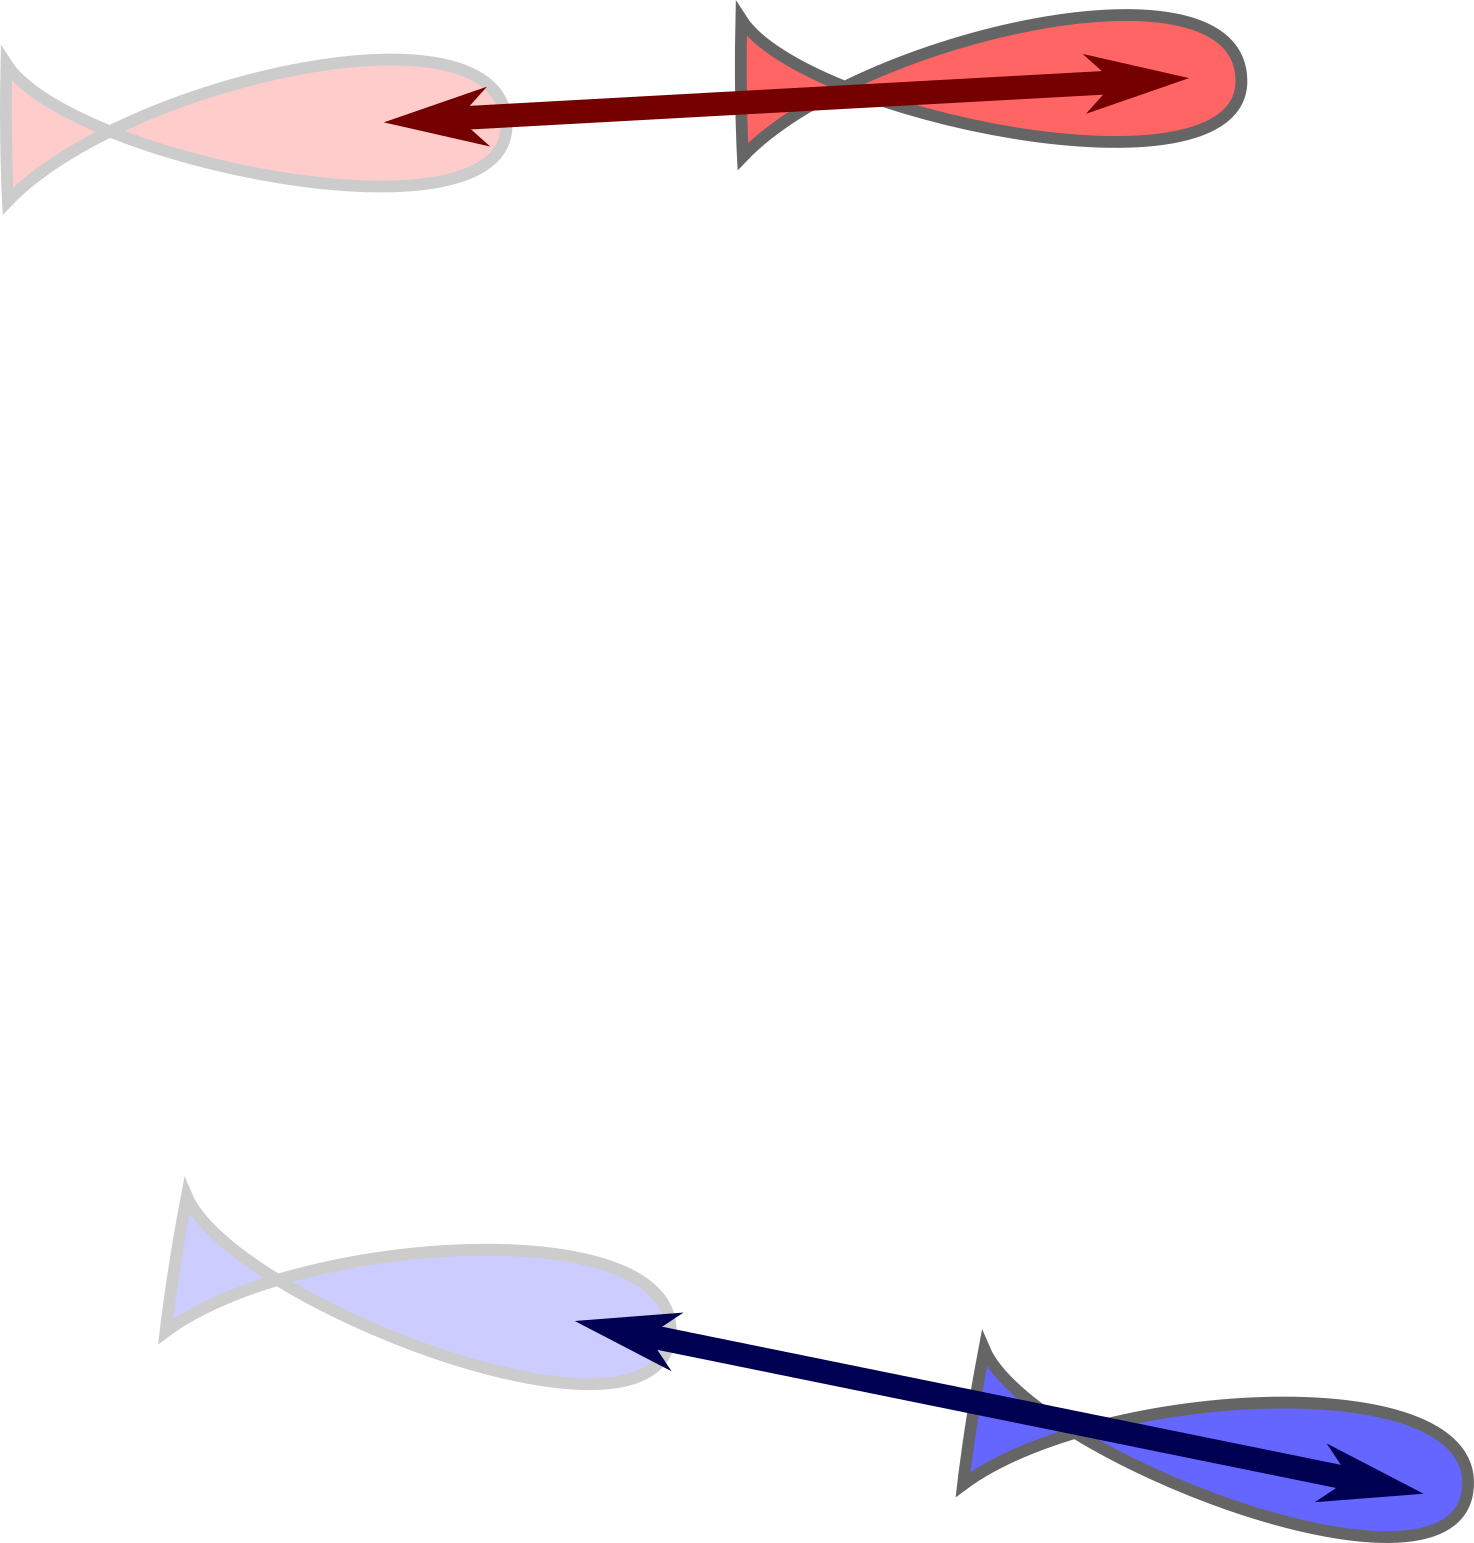
\includegraphics[width=0.4\linewidth]{distance-swap1}
	\hspace{0.05\linewidth}
	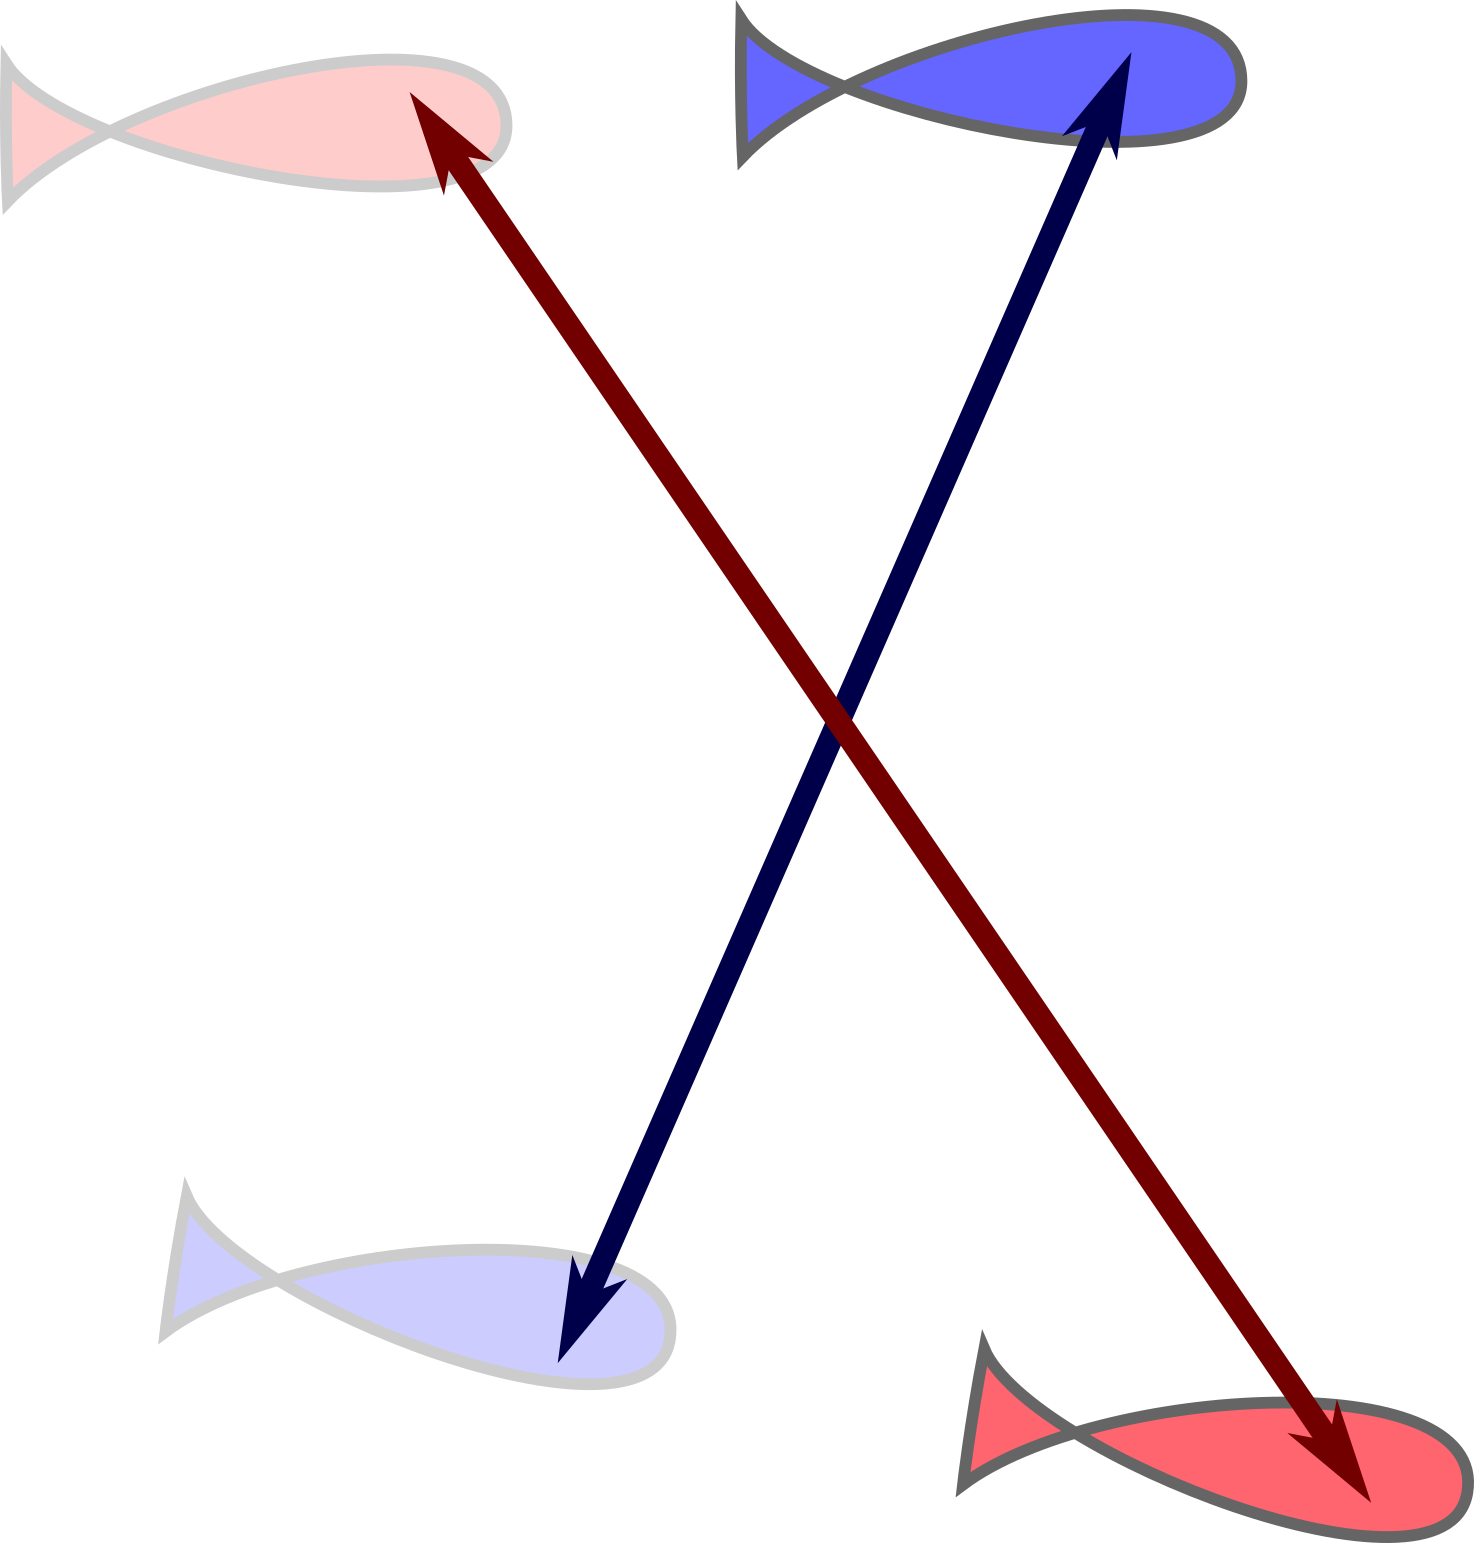
\includegraphics[width=0.4\linewidth]{distance-swap2}
	\caption{Distance traveled by the fish between two frames when identities are maintained (left panel) and when identities are swapped (right panel).}
	\label{fig:distance-unswap-principle}
\end{figure}

In order to determine whether a swap has occurred, we compute the following distance matrix, which contains all four of the distances shown in the figure:
%
\newcommand{\myMatrixItem}[1]{\begin{minipage}[b]{15em}\singlespacing{#1}\end{minipage}}
\begin{equation}
	\begin{pmatrix}
		\text{\myMatrixItem{distance from fish 1 in previous \\ frame to fish 1 in current frame}} 
			& \text{\myMatrixItem{distance from fish 1 in previous \\ frame to fish 2 in current frame}} 
		\\
		\text{\myMatrixItem{distance from fish 2 in previous \\ frame to fish 1 in current frame}} 
			& \text{\myMatrixItem{distance from fish 2 in previous \\ frame to fish 2 in current frame}} 
	\end{pmatrix}
	\nonumber
\end{equation} 
%
The sum of the diagonal terms (previous-1-to-current-1 and previous-2-to-current-2) represents the total distance traveled by both fish since the previous frame assuming identities were maintained. The sum of the two off-diagonal terms (previous-1-to-current-2 and previous-2-to-current-1) represents the total distance traveled by both fish since the previous frame assuming identities were swapped. If the latter is smaller than the former, then we conclude the identities were swapped.

%\begin{figure}[H]
%	\centering
%	\includegraphics[width=.75\linewidth]{fish2}
%	\caption{Basic overview of unswapping logic}
%\end{figure}


\subsection{Histogram Based Unswapping}
\label{sec:Histogram Based Unswapping}

When the two fish overlap, the distance-based method described above no longer works, and a new method is required. Following idTracker~\cite{perez-escudero_idtracker_2014}, we compute a visual signature of each fish based on the brightness correlations. Figure~\ref{fig:brightness-correlation} illustrate the basic principle of the method. 

\begin{figure}[H]
	\centering
	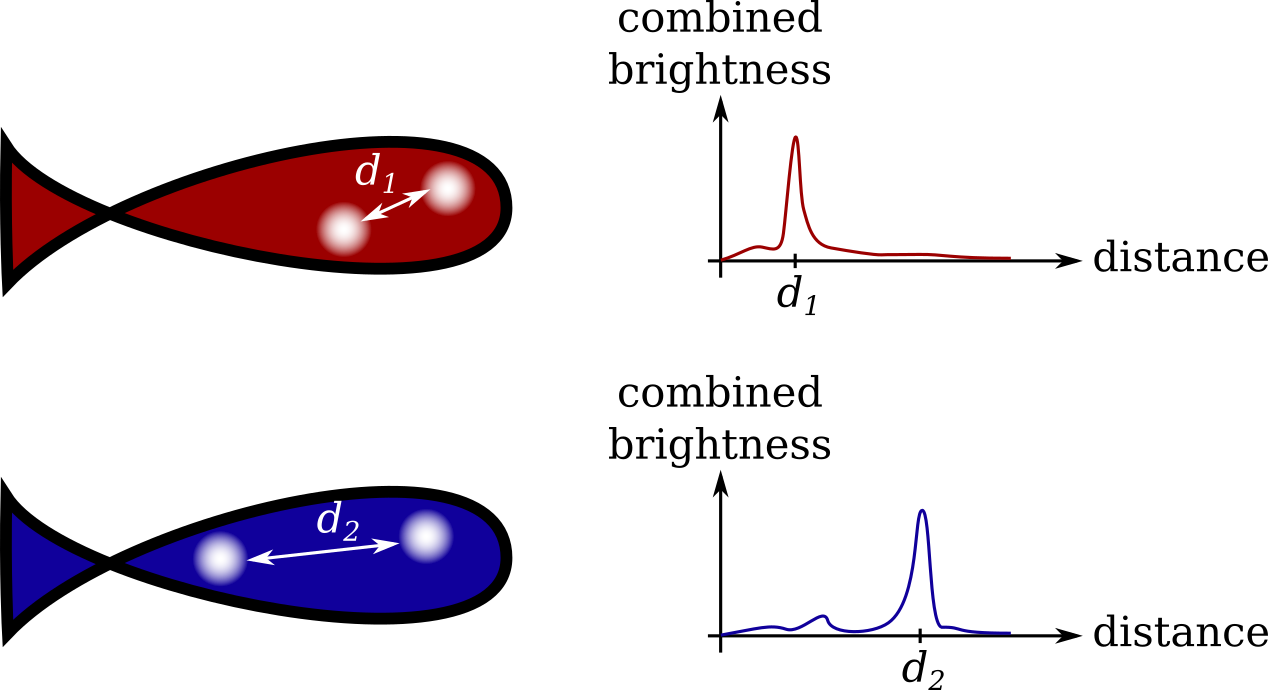
\includegraphics[width=0.6\linewidth]{brightness-correlation}
	\caption{An example of how the brightness map is used to identify the fish}
	\label{fig:brightness-correlation}
\end{figure}

It looks at the cumulative brightness of every pair of pixels on a fish's body and computes the chances of finding a specific cumulated brightness at a specific distance. As an example, consider a fish with two bright spots separated by a distance $d$. Then the chance of finding two pixels with a large cumulated brightness and a distance $d$ between them is higher. This translates to a peak in the combined brightness vs distance graph. The location of such peaks can then be used to identify a fish, and ultimately decide whether two fish from different frames are the same fish or not. 

The actual method used in~\cite{perez-escudero_idtracker_2014} and in our code uses a slightly more detailed description of brightness correlations. For each inter-pixel distance, we log not only the average cumulated brightness, but the chances of getting various values of the cumulated brightness. The result is the 2d histogram shown in Figure~\ref{fig:singleHist}.

\begin{figure}[H]
	\centering
	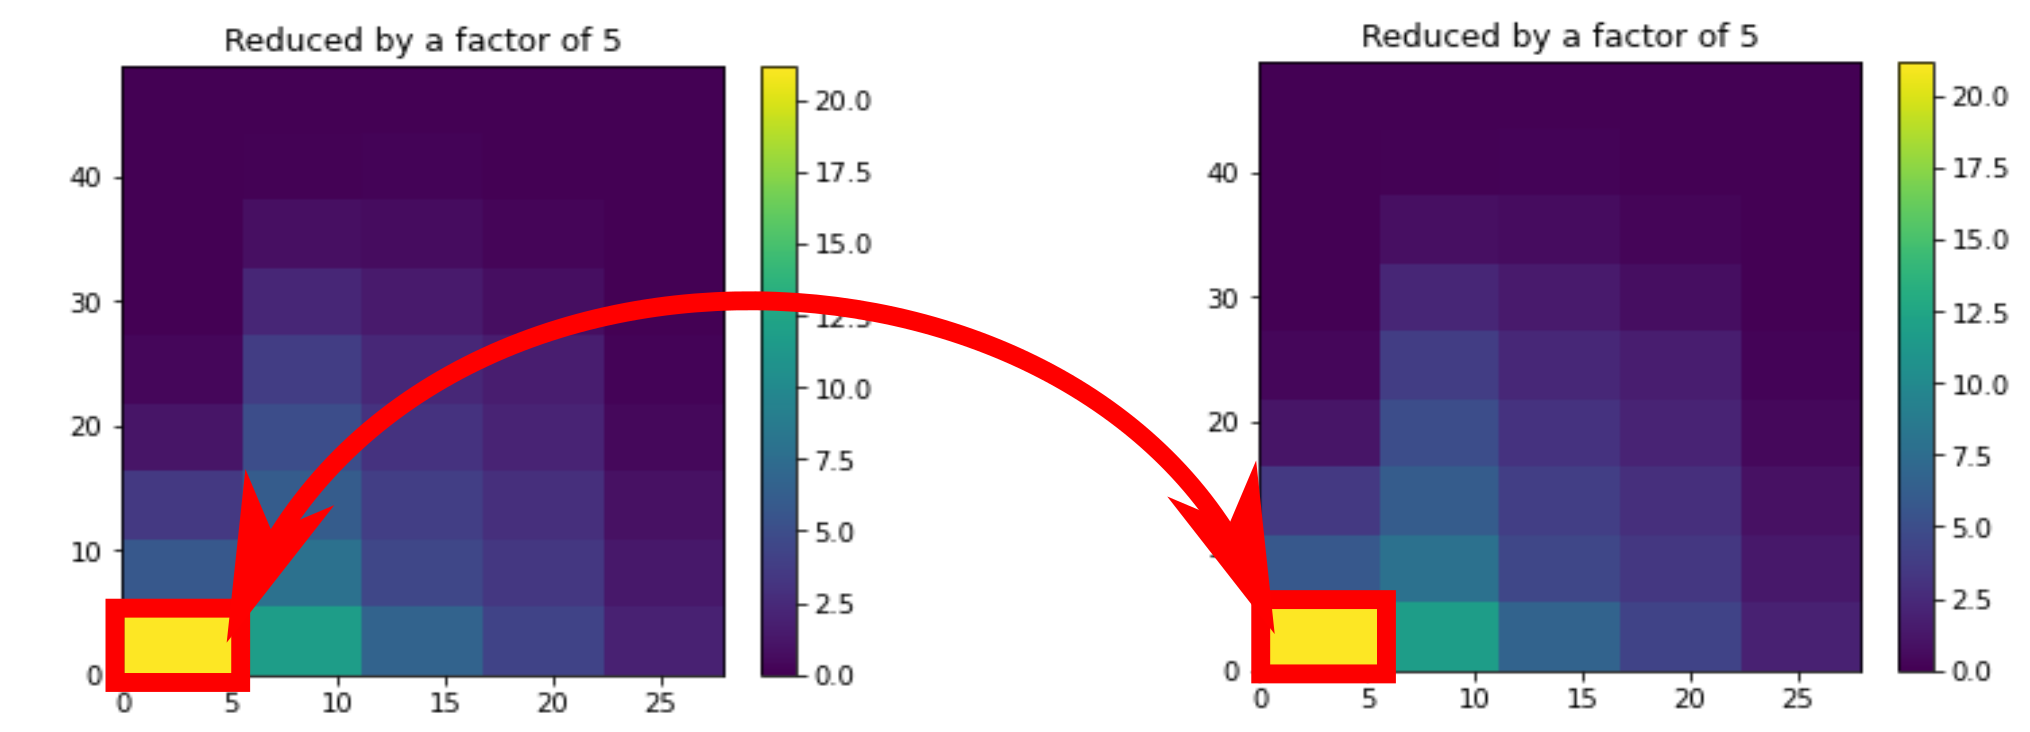
\includegraphics[width=\linewidth]{twoHist}
	\caption{Brightness correlation as a visual identifier of the fish. To decide whether two histograms are from the same fish, the histograms are compared bin by bin (red arrow), and then these values are added to provide values.}
	\label{fig:singleHist}
\end{figure}

The next step is to define the similarity metric to assess whether two 2d brightness histograms are likely to be the same fish or not. To do this, we compare bin heights in the two histograms one bin at a time (red arrow in Figure~\ref{fig:singleHist}). We then add up the squares of all those bin heights and take the square root. In other words, we compute the Euclidean distance between the two histograms.

Finally, we compute the distance matrix as in section~\ref{sec:Distance Based Unswapping}, except the distance is now the distance between the histograms rather than the physical distance between the fish:
%\newcommand{\myMatrixItem}[1]{\begin{minipage}[b]{15em}\singlespacing{#1}\end{minipage}}
\begin{equation}
	\begin{pmatrix}
	\text{\myMatrixItem{distance between histogram 1 in \\ previous frame and histogram 1 \\ in current frame}} 
	& \text{\myMatrixItem{distance between histogram 1 in \\ previous frame and histogram 2 \\ in current frame}} 
	\\
	\text{\myMatrixItem{distance between histogram 2 in \\ previous frame and histogram 1 \\ in current frame}} 
	& \text{\myMatrixItem{distance between histogram 2 in \\ previous frame and histogram 2 \\ in current frame}} 
	\end{pmatrix}
	\nonumber
\end{equation} 
where \emph{histogram 1} is the 2d histogram computed obtained from fish 1 and \emph{histogram 2} is the one obtained from fish 2.
As in the distance-based method, if the sum of the diagonal terms is larger than the sum of the off-diagonal terms, we conclude that a swap has occurred.


\subsection{A Basic Overview of Analysing Histograms}
\label{sec:Histogram Based Unswapping 2}

As the histogram based unswapping method only works in time frames of the video in which there are two fish detected, the regions with only one fish detected must be identified so that the histogram unswapping method can be used to reidentify the fish after the overlap (see figure~\ref{fig:nonoverlappingRange}). The approach that was used for determining these overlapping regions was to comb through the list of the fish in each frame for the amount of fish that the program detected (see Appendix~\ref{appendix1}).

\begin{figure}[H]
	\centering
	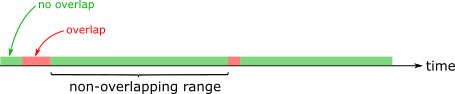
\includegraphics[width=\linewidth]{nonoverlappingRange}
	\caption{The nonoverlapping ranges}
	\label{fig:nonoverlappingRange}
\end{figure}

The big advantage of histogram-based unswaps compared to distance-based unswapping is that it can reidentify the fish even after an extended period of time, regardless of the distance traveled by the fish during that time.

\subsection{Determining Accuracy}
\label{sec:Determining Accuracy}

The distance-based method is widely used and known to work well, so we concentrate our efforts on the histogram based unswaps. First, we established the true identities of the fish by hand by watching the video through the first 60 overlaps. The accuracy rate was then obtained by measuring the percentage of overlaps after which the program correctly guessed whether there had been a swap.

\section{Results}
\label{sec:Results}

%\subsection{Distance Based Unswapping}

%\subsection{Histogram Based Unswapping and Bin Reduction}

The main question when constructing the combined brightness histograms is how to choose the bins. The size of the fish is less than 30 pixels, so the distance between two pixels on the same fish is always smaller than 30 pixels, and the distance bins only need to go up to 30 pixels. That distance, however, can go all the way down to 1 pixel when comparing two neighboring pixels. The range of typical values for the combined brightness (the vertical axis of the histogram) was initially set to $0\rightarrow510$, because individual pixel brightness values are in the range $0\rightarrow255$. This range was then reduced to $150\rightarrow350$ (for brightness sum histogram) or $0\rightarrow50$ (for brightness difference histograms) based on the values actually encountered in the video of interest.

The width of the bins (or equivalently the number of bins) also plays a role. Too many bins increases the noise. Not enough bins makes all fish look the same. To find the ideal bin width, we started with a narrow bin width then produced ``reduced'' histograms by merging bins together as shown in Figure~\ref{fig:reducedHist}.

\begin{figure}[H]
	\centering
	\includegraphics[width=\linewidth]{reducedHist2}
	\caption{Bin reduction. ``Reduced by a factor of $n$'' means that a square of $n\times n$ original bins were merged to form the new bins.}
	\label{fig:reducedHist}
\end{figure}



To find the ideal bin width, we tested several widths and computed the accuracy of each. 
Figure~\ref{fig:error-rate} shows which overlaps led to a an identity swap (red crosses) and which ones did not (green circles). The upper line shows true swaps as based on identifying the fish by eye. The lower line shows when the histogram-based algorithm detected a swap. The error rate in this case is $19\%$, meaning that in $19\%$ of overlaps the algorithm either thought there was a swap when there wasn't or thought there was no swap when there was. 
Varying the bin size made little difference.

\begin{figure}[H]
	\centering
	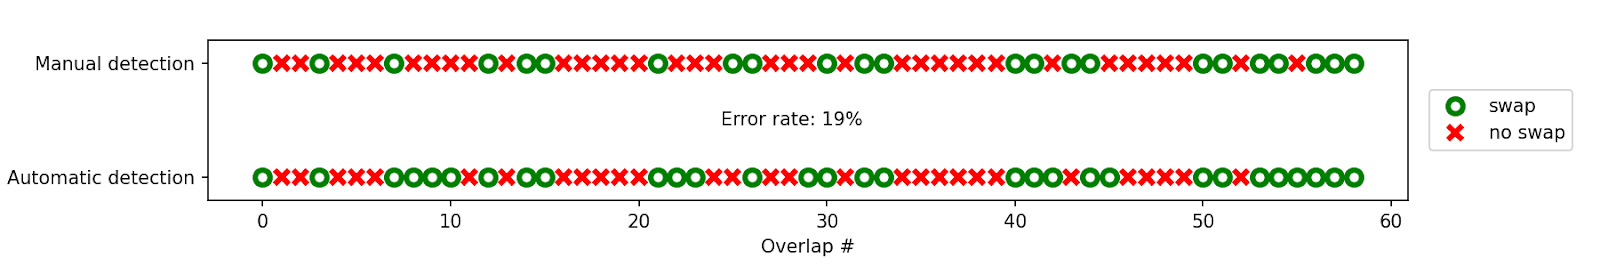
\includegraphics[width=\linewidth]{error}
	\caption{The error of the untuned process}
	\label{fig:error-rate}
\end{figure}



%One thing that was also tested was what would happen if less bins were used on the histograms used for analysis, both to see how it affected accuracy and performance. What was found was that there was no significant change in the accuracy of the data when this operation was performed. The most difference in accuracy between the reduced and nonreduced datasets that we were able to observe was 13\%, with that being an outlier considering most reductions were under 9\%, with the vast majority being under 6\%. 


\section{Conclusion}

One problem faced by scientists working on animal tracking tasks is keeping track of which animal is which. To solve this problem for the Jupiter Trilab, we aimed to create a software that detects fish based on a unique identifier. To do this, first we looked at the two types of identity swaps that occur in the original software: a first type that can be fixed by analysing the distance traveled by the fish from frame to frame, and a second type where the fish are so close to each other that the image recognition software only sees one fish. For the second of these swaps, we took the visual identifier of the brightness histogram of each fish and used that to determine the fish's identities. When combined, the two methods perform reasonably well, but not well enough, correctly re-identifying the fish about 80\% of the time after they crossed path. 

In retrospect, the video used to develop the program is particularly challenging for two reasons. First, each fish occupies a relatively small number of pixels, about 100 pixels on average. Increasing the video's resolution would provide more visual detail for the histogram-based method to analyze.
Second, the fish's skin has a fairly uniform dark color, which makes it more difficult to pick up patterns of brightness to identify them. Some of the other fish used in the CaveFish Trilab are partially transparent, which may lead to a greater variety of brightness values over each fish's body, and more information for the histogram-based method to pick up.


\appendix
\section{Locating Nonoverlapping Ranges}
\label{appendix1}

\begin{minipage}[c]{\textwidth}
\begin{lstlisting}[language=Python]
i2=0
nonOverlappingRange=[]
while i2<len(fish):
    i1=i2
    while i1<len(fish) and len(fish[i1])!=2:
        i1+=1
    i2=i1
    while i2 < len(fish) and len(fish[i2])==2:
        #find the first overlapping index
        i2+=1
    nonOverlappingRange.append([i1,i2])
print(nonOverlappingRange)
\end{lstlisting}
\end{minipage}

\section{Distance Based Swap Checking}
\label{app:swapStatus}

\begin{lstlisting}[language=Python]
def swapStatus(pos,i):
    '''
    Detect swaps between consecutive frames based on proximity.
    
    Input:
        pos:Postionts. Array with shape (Nframes,Nfish,Ndimensions),
        i: Frame index. Int.
    
    Output:
        Int. 0 if no swaps, 1 if swapped, 2 if overlapping.
    '''
    nFish=pos.shape[1] #Number of fish
    distanceMatrix=[np.linalg.norm(pos[i+1][0]-pos[i][0]),
                    np.linalg.norm(pos[i+1][1]-pos[i][1]),
                    np.linalg.norm(pos[i+1][0]-pos[i][1]),
                    np.linalg.norm(pos[i+1][1]-pos[i][0])]
    swapCriteron=(distanceMatrix[0]+distanceMatrix[1])-(distanceMatrix[2]+distanceMatrix[3])
    if abs(swapCriteron)<1e-10:
        return 2 #Overlapping
    elif swapCriteron>0:
        return 1 #Swapped
    elif swapCriteron<0:
        return 0 #Normal
    else:
        return -1
\end{lstlisting}

\section{Data Shape}
\label{app:dataShape}

The data is stored in an array of shape [frame][fish][xpixels,ypixels][color]

\begin{figure}[H]
	\centering
	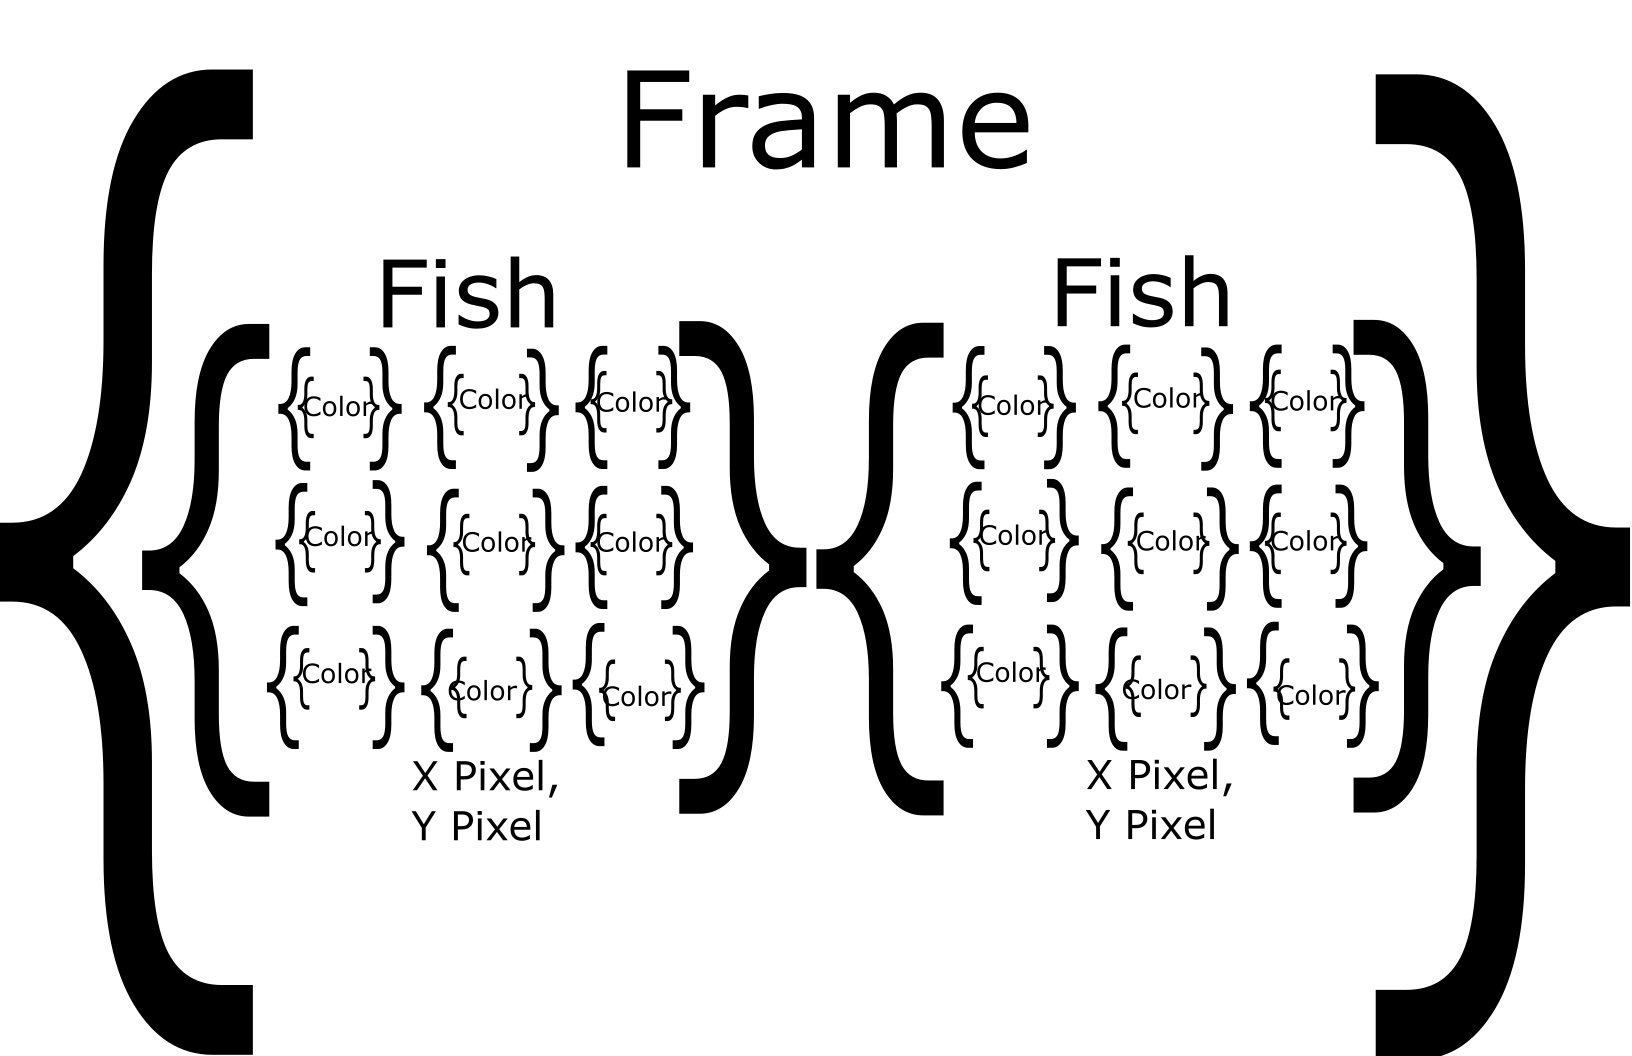
\includegraphics[width=\linewidth]{array}
	\caption{The shape of the array that holds the data}
	\label{fig:array}
\end{figure}


\section{Histogram Creation}
\label{app:histCreator}

\begin{lstlisting}[language=Python]
for i in tnrange(60,desc='nonOverlappingRange'):
    for k in range(2):
        countSum=0
        countDif=0
        pairData=[]
        for j in range(*nonOverlappingRange[i]):
            fishPixels = fishU[j][k]
            m,l=np.triu_indices(fishPixels.shape[0],k=1)
            d=np.sqrt((fishPixels[l,0]-fishPixels[m,0])**2+(fishPixels[l,1]-fishPixels[m,1])**2)
            bSum=fishPixels[l,2]+fishPixels[m,2]
            bDif=fishPixels[l,2]-fishPixels[m,2]

            heightValuesSum,_,_=np.histogram2d(d,bSum,bins=(binsDist,binsSum))
            histSum+=heightValuesSum
            countSum+=1
            heightValuesDif,_,_=np.histogram2d(d,bDif,bins=(binsDist,binsDif))
            histDif+=heightValuesDif
            countDif+=1
        histSum/=countSum
        histSumList[i,k]=histSum.copy()
        histDif/=countDif
        histDifList[i,k]=histDif.copy()
\end{lstlisting}

%==========================================================================
% Bibliography.

\bibliographystyle{plain}
\bibliography{fish}


\end{document}
